% % % % % % % % % % % % % % % % % % % % % % % % % % % % % % % % 
% BSc Physics Dissertation
% % % % % % % % % % % % % % % % % % % % % % % % % % % % % % % %
\documentclass[twoside, fontsize=12pt,
     bibliography=totoc, % Include bibliography in contents
     listof=totoc, % Include lists of figures and tables in contents
     index=totoc, % Include index in contents
     onehalfspacing %  or doublespacing
    %,openright
]{_MScDiss2017_cls}

%\usepackage{txfonts,epsfig}
\usepackage[labelfont=footnotesize,textfont=footnotesize]{caption}   
\usepackage{_twoopt}
\usepackage{url}
\usepackage[colorlinks,citecolor=blue,linkcolor=blue,urlcolor=blue,hyperfootnotes=false,linktocpage,breaklinks=true]{hyperref}
%\usepackage{breakurl}
\usepackage[]{_MScDiss_sty}
%\usepackage{chngcntr}
%\counterwithout{footnote}{chapter}

%% these macros turn citations into ADS clickers in dvi, pdf, html output
%% (EDP Sciences improved them in December 2012 to work also with pdflatex)
\bibpunct{(}{)}{;}{a}{}{,}    %% natbib cite format used by A&A and ApJ
\makeatletter
 \newcommandtwoopt{\citeads}[3][][]{\href{http://adsabs.harvard.edu/abs/#3}%
   {\def\hyper@linkstart##1##2{}%
    \let\hyper@linkend\@empty\citealp[#1][#2]{#3}}}    %% Rutten, 2000
 \newcommandtwoopt{\citepads}[3][][]{\href{http://adsabs.harvard.edu/abs/#3}%
   {\def\hyper@linkstart##1##2{}%
    \let\hyper@linkend\@empty\citep[#1][#2]{#3}}}      %% (Rutten 2000)
 \newcommandtwoopt{\citetads}[3][][]{\href{http://adsabs.harvard.edu/abs/#3}%
   {\def\hyper@linkstart##1##2{}%
    \let\hyper@linkend\@empty\citet[#1][#2]{#3}}}      %% Rutten (2000)
 \newcommandtwoopt{\citeyearads}[3][][]%
   {\href{http://adsabs.harvard.edu/abs/#3}%
   {\def\hyper@linkstart##1##2{}%
    \let\hyper@linkend\@empty\citeyear[#1][#2]{#3}}}   %% 2000
\makeatother

\declaration{I hereby certify that this Dissertation, which is approximately N thousand words in length, has been written by me at the School of Physics and Astronomy, Queen Mary University of London, that all material in this dissertation which is not my own work has been properly acknowledged, and  that it has not been submitted in any previous application for a higher degree.} 

%--Put your information between here----%
\title{The Effects of Neutrinos on the CMB Power Spectrum}
\author{Daniil Dolgich (150066826)}
\supervisor{Prof. Teppei Katori}
\date{\today}
%\date{July 2019} 
\acknowledgements{I  thank whoever I want here - or I can instead comment it out.}
\newpage % to ensure page 1 starts on front of a page rather than back
%%---and here------%

\begin{document}
\pagenumbering{roman}
\setcounter{tocdepth}{5}

\maketitle
\abstract{The origin of the Universe is modeled.}
\tableofcontents % generates Table of Contents
\listoffigures % generates List of figures
\listoftables % generates List of Tables

\newpage% to flush out last roman numeral
\cleardoublepage
\pagenumbering{arabic}% Set arabic page numbers now that dissertation proper is starting.

% rather than having a very long file you can Input files for each chapter/section here using 
% \input{relative-path-to-file} or just put the files in the same directory as this file.

%Chapter
\chapter{The Dissertation Template}

\label{sec:template}

\begin{figure}[hbtp]
  \begin{center}
  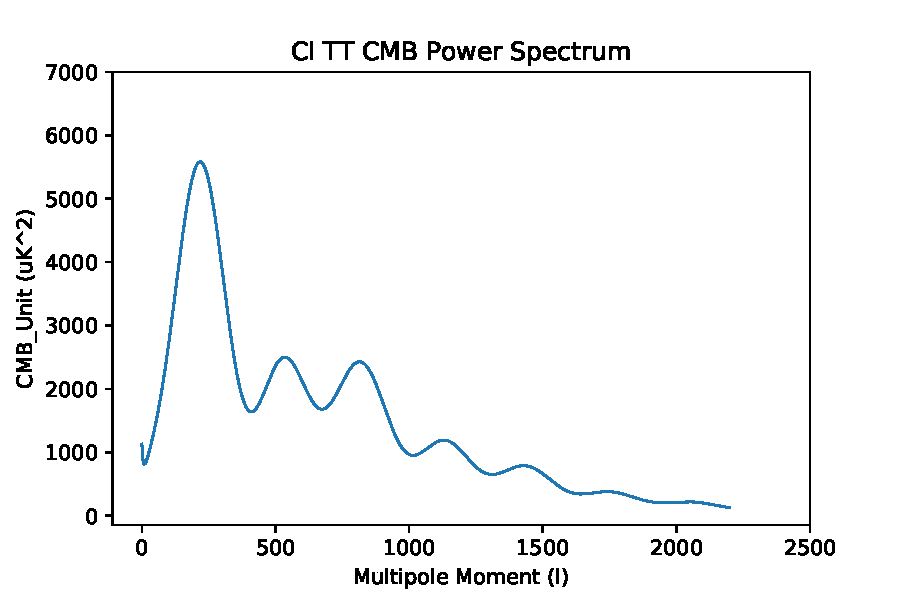
\includegraphics[width=80mm]{Cl-TT-vs-l.pdf}
  \caption{Scalar Non-lensed CMB Power Spectrum Cl\^ TT} 
  \label{fig:texworks-prefs}
  \end{center}
\end{figure}

%%BIBLIOGRAPHY SECTION
\begin{singlespace}% Start single space for bibliography
\bibliographystyle{_abbrvnat_jpe}    
\bibliography{Surname,bib-aanda,bib-apj,bib-astronj,bib-mnras,bib-stateqm,bib-various} %makes BIBLIOGRAPHY from the listed bib files  
\end{singlespace}

\end{document}
